\chapter[SCP-081 人体自燃病毒]{
    SCP-081 Spontaneous Combustion Virus\\
    SCP-081 人体自燃病毒
}

\label{chap:SCP-081}

\begin{figure}[H]
    \centering
    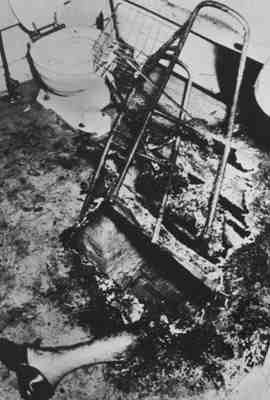
\includegraphics[width=0.4\linewidth]{images/SCP.081.jpg}
    \caption*{发展到SCP-081的第四阶段后的Mary Reeser的尸体。}
\end{figure}

\bb{项目编号:}SCP-081

\bb{项目分类:}Euclid

\bb{特殊收容措施:}只有拥有4级权限和有███████的书面批准的人才可接近SCP-081。在收容区域内必须随时身着全套防护装备,包括有防护服、手套和一个氧气罐。在离开收容区域之前,必须对防护服喷洒消毒液。一旦收容失效,整个收容区域必须要进行紫外线消毒,随后漂白。被怀疑已感染的人员必须至少隔离十(10)天,当十天之后仍没有出现感染的症状,方可解除隔离。

\bb{描述:}SCP-081是一种有传染性的病毒,似乎是███████病毒的突变种,但它的RNA有█个片段而不是█个。此病毒只感染人类,但老鼠是其载体和传播者。SCP-081也可通过性接触和接触已感染的血液来传播。

SCP-081在感染了脂肪细胞和白细胞后会迅速地吸收其营养。在营养被吸收完后,被感染了的B细胞会生产、分泌大量的被改动了的人类抗体。随后脂肪细胞将变大且开始增生,随之机体的热量摄入量也在增加。在机体内的脂肪浓度达到一个临界值时,病毒引发产生的抗体会促使全身的细胞裂解,这会导致此后被感染个体自发地燃烧起来。

在感染后到最初的症状出现前有一(1)周的潜伏期。症状持续的时间完全由被感染者身体的脂肪率来决定。感染过程分为如下四(4)个明显的阶段。

\begin{itemize}
\item \bb{第一阶段:}在第一周不会有明显的主要症状,但测试者偶尔会反映有些疲倦。
\item \bb{第二阶段:}在感染后的第二周,测试者会出现“潮热”以及食欲变大的情况。
\item \bb{第三阶段:}被感染的测试者表现出拥有极大的食量。他们会做任何事情来试图获取食物甚至于任何能吃的东西。在这个阶段,测试者的新陈代谢率明显下降,体重快速上升。从本阶段到第四和最终阶段(原文没有最终阶段,推测此处指自燃\footnote{\bb{译注:}资料来源不明})之间没有固定的间隔时间。病毒为了完成其生命周期,至少会促使被感染者身体的脂肪率达到55\%。
\item \bb{第四阶段:}一旦测试者身体的脂肪率达到了55\%,他们进食的强烈欲望将会停止,但测试者报告“潮热”的次数会变得越来越多。很快测试者的身体就会出现极其剧烈的细胞裂解。随着细胞的炸裂,被改动了的抗体开始催化脂肪组织通过未知的方法燃烧起来。通过烛芯效应,测试者的身体会由内到外烧成灰烬,多余的脂肪在其中起到了燃料的作用。鉴于第四阶段没有大的临床症状,测试者无法预知燃烧将于何时开始,显然的,准确发生的时间是随机的。
\end{itemize}

\bb{附录081-1:}历史上有记载的第一起SCP-081导致的病例是由法国的Jonas Dupont(约拿斯•杜朋)在1673年记录下的。在他所著的《De Incendiis Corporis Humani Spontaneis》里,他描述了一个一位法国男性被控杀妻的案例,他在陪审团一致同意其妻死于人体自燃后被宣判无罪。需注意上述的女性死亡时严重地超重。直到1951年7月2日时Mary Reeser的死亡,基金会才注意到了SCP-081的存在。尽管基金会做出了努力,此消息仍通过图片的形式泄露到了公众传媒里。我们相信大部分报道里的自燃案例都是由SCP-081引起的。

\bb{附录081-2:}据推测SCP-081自9██年起就存在,现认为其起源于█████████████。鉴于当时许多欧洲国家都普遍存在饥饿和营养不良的问题,发展到第三、四阶段的SCP-081感染者很罕见。上世纪的大多数的SCP-081感染者都出现在北美洲,不过由于环境的改善和积极的灭鼠活动,SCP-081的病例已显著下降。每年只有不到███人死于SCP-081的后期阶段。

\bb{附录081-3:}鉴于目前美国肥胖人数过多,根除野生SCP-081便显得十分重要。若SCP-081大规模流行则会导致其信息向公众暴露,这对成功的收容措施的影响将是灾难性的。-██████████博士。

\bb{附录081-4:}在试验中已发现,糖尿病患者自身对SCP-081免疫。但这项发现并没有为寻求治疗此病毒的方法的发展有所帮助,它仍然无法被治愈。野外的感染{[}数据删除],并提供另一种死亡原因\footnote{\bb{译注:}以供掩饰}。

\bb{附录081-5:}\ii{特工█████发现,SCP-081可通过暴露在已死亡感染者的灰烬前传播。收容和流行病防控预案正在修订,回应了█████████女士的求助电话的急救人员已被拘留以进行评估。}-██████████博士。
